% !TeX spellcheck = en_US
% !TeX encoding = utf8
% !TeX program = xelatex
% !BIB program = bibtex

% \documentclass[notes]{beamer}
\documentclass[draft]{beamer}	
\usetheme{Hannover}
% \usecolortheme{default}
%\usepackage{pgfpages}
%\setbeameroption{show notes on second screen}

\usepackage[british]{babel}
\usepackage{graphicx,hyperref,url}
% \usepackage{ru}
\usepackage{mmstyles}
% \usepackage{hanging}
\usepackage{listings}
\usepackage{fontspec}
\usefonttheme[onlymath]{serif}
\usepackage{xeCJK}
% \usepackage[backend=biber]{biblatex}
% \bibliography{./ref.bib}
%\addbibresource{ref.bib}
\usepackage{indentfirst}
\usepackage{longtable}
\usepackage{float}
%\usepackage{picins}
\usepackage{rotating}
\usepackage{subfigure}
\usepackage{tabu}
\usepackage{amsmath}
\usepackage{amssymb}
\usepackage{setspace}
\usepackage{amsfonts}
\usepackage{appendix}
\usepackage{listings}
\usepackage{xcolor}
\usepackage{geometry}
% \setCJKfamilyfont{cjkhwxk}{SimSun}
% \newcommand*{\cjkhwxk}{\CJKfamily{cjkhwxk}}
%\newfontfamily{\consolas}{Consolas}
%\newfontfamily{\monaco}{Monaco}
%\setmonofont[Mapping={}]{Consolas}	%英文引号之类的正常显示,相当于设置英文字体
%\setsansfont{Consolas} %设置英文字体 Monaco, Consolas,  Fantasque Sans Mono
% \setmainfont{Times New Roman}
% \newfontfamily{\consolas}{Times New Roman}
% \newfontfamily{\monaco}{Arial}
% \setCJKmainfont{Times New Roman}
%\setmainfont{MONACO.TTF}
%\setsansfont{MONACO.TTF}
\newcommand{\verylarge}{\fontsize{60pt}{\baselineskip}\selectfont}  
\newcommand{\chuhao}{\fontsize{44.9pt}{\baselineskip}\selectfont}  
\newcommand{\xiaochu}{\fontsize{38.5pt}{\baselineskip}\selectfont}  
\newcommand{\yihao}{\fontsize{27.8pt}{\baselineskip}\selectfont}  
\newcommand{\xiaoyi}{\fontsize{25.7pt}{\baselineskip}\selectfont}  
\newcommand{\erhao}{\fontsize{23.5pt}{\baselineskip}\selectfont}  
\newcommand{\xiaoerhao}{\fontsize{19.3pt}{\baselineskip}\selectfont} 
\newcommand{\sihao}{\fontsize{14pt}{\baselineskip}\selectfont}      % 字号设置  
\newcommand{\xiaosihao}{\fontsize{12pt}{\baselineskip}\selectfont}  % 字号设置  
\newcommand{\wuhao}{\fontsize{10.5pt}{\baselineskip}\selectfont}    % 字号设置  
\newcommand{\xiaowuhao}{\fontsize{9pt}{\baselineskip}\selectfont}   % 字号设置  
\newcommand{\liuhao}{\fontsize{7.875pt}{\baselineskip}\selectfont}  % 字号设置  
\newcommand{\qihao}{\fontsize{5.25pt}{\baselineskip}\selectfont}    % 字号设置 

\graphicspath{{./fig/}}

% \setbeamertemplate{footnote}{%
%   \hangpara{2em}{1}%
%   \makebox[2em][l]{\insertfootnotemark}\footnotesize\insertfootnotetext\par%
% }

\definecolor{cred}{rgb}{0.6,0,0}
\definecolor{cgreen}{rgb}{0.25,0.5,0.35}
\definecolor{cpurple}{rgb}{0.5,0,0.35}
\definecolor{cdocblue}{rgb}{0.25,0.35,0.75}
\definecolor{cdark}{rgb}{0.95,1.0,1.0}
\lstset{
	language=R,
	numbers=left,
	numberstyle=\tiny\color{black},
	keywordstyle=\color{cpurple}\consolas,
	commentstyle=\color{cgreen}\consolas,
	stringstyle=\color{cred}\consolas,
	frame=single,
	escapeinside=``,
	xleftmargin=1em,
	xrightmargin=1em, 
	backgroundcolor=\color{cdark},
	aboveskip=1em,
	breaklines=true,
	tabsize=3
} 
% The title of the presentation:
%  - first a short version which is visible at the bottom of each slide;
%  - second the full title shown on the title slide;
\title[Opt for ML]{Optimization for Machine Learning}

% Optional: a subtitle to be dispalyed on the title slide
\subtitle{Introduction}

% The author(s) of the presentation:
%  - again first a short version to be displayed at the bottom;
%  - next the full list of authors, which may include contact information;
\author[YingmingLi]{Yingming Li \\ yingming@zju.edu.cn}
% The institute:
%  - to start the name of the university as displayed on the top of each slide
%    this can be adjusted such that you can also create a Dutch version
%  - next the institute information as displayed on the title slide

\institute[DSERC, ZJU]{Data Science \& Engineering Research Center, ZJU}

% Add a date and possibly the name of the event to the slides
%  - again first a short version to be shown at the bottom of each slide
%  - second the full date and event name for the title slide
\date[\today]{\today}

\begin{document}

\begin{frame}
  \titlepage
\end{frame}

\AtBeginSection[]
{
   \begin{frame}
       \frametitle{Outline}
       \tableofcontents[currentsection]
   \end{frame}
}

% \AtBeginSubsection[2-]
% {
%    \begin{frame}
%        \frametitle{Outline}
%        \tableofcontents[currentsection]
%    \end{frame}
% }

\section{What is optimization?} 
% \subsection{Examples in machine learning} 
% \subsection{Unconstrained vs constrained} 

\begin{frame}{What is optimization?}
	\begin{itemize}
		\item<1-> Finding (one or more)  minimizer of a function subject to constraints 
			\begin{equation}
			\begin{aligned}
				\argmin_x \quad & f_0(x)  \\ 
				\textrm{s.t.} \quad & f_i(x) \le 0, i = \{1,...,k\} \\  
				 		\quad & h_j(x) = 0, j = \{1,...,l\} \\ 
			\end{aligned}
			\end{equation}
		\item<2-> Most of the machine learning problems are, in the end, optimization problems. 
	\end{itemize}
\end{frame}	

\begin{frame}{Examples} 
	\begin{itemize} 
		\item (Soft) Linear SVM 
		\begin{equation}
			\begin{aligned}
				\argmin_x \quad & \sum_{i=1}^{n} \|w\|^2 + C \sum_{i=1}{n} \epsilon_i  \\ 
				\textrm{s.t.} \quad & 1-y_ix_i^Tw\le \epsilon_i \\  
				 		\quad & \epsilon_i \ge 0 \\ 
			\end{aligned}
		\end{equation}
		\item Maximum Likelihood 
		\begin{equation}
			\argmax_\theta \sum_{i=1}^{n} \log p_\theta (x_i)
		\end{equation}
		\item K-means 
		\begin{equation}
			\argmin_{\mu_1,\mu_2,...,\mu_k} J(\mu) = \sum_{j=1}^{k} \sum_i\in C_j \|x_i-\mu_j\|^2 
		\end{equation}
	\end{itemize}
\end{frame}

\section{Convex optimization} 
\subsection{Convex sets} 

\begin{frame}{Convex sets}
\begin{define}
A set $C \subseteq \real^n$ is convex if for $x,y \in C$ and any $\alpha \in [0,1]$, $\alpha x +(1-\alpha)y \in C$. 
\end{define}
\begin{figure}
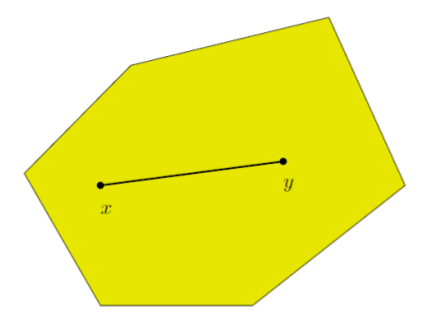
\includegraphics[width=.45\textwidth]{2018-03-04-21-52-01.png} 
\caption{Convex Set}
\end{figure}

\end{frame}

\begin{frame}{Convex sets} 
	\begin{example}
		\begin{itemize}
			\item All of $\real^n$
			\item Non-negative orthant, $\real_+^n$: let $x \ge 0, y\ge 0$, clearly $\alpha x + (1-\alpha) y \ge 0$. 
			\item Afline subspaces: $Ax=b, Ay=b$, then 
			$$A(\alpha x+(1-\alpha) y)=\alpha Ax + (1-\alpha)Ay = b$$. 
			\item Aebitrary intersections of convex sets: let $C_i$ be convex for $i\in \cI, C = \bigcap_i C_i$, then 
			$$x\in C,y\in C \Rightarrow \alpha x +(1-\alpha y) \in C_i \subseteq C, \forall i \in \cI $$.
		\end{itemize}
	\end{example}
\end{frame}

\subsection{Convex functions} 
\begin{frame}{Convex functions} 
	\begin{define}
		A function $f: \real^n \rightarrow \real$ is convex if  for $x,y \in \text{dom } f$ and any $a\in [0,1]$, 
		$$f(ax+(1-a)y)\le af(x)+(1-a) f(y)$$
	\end{define}
	\begin{figure}
	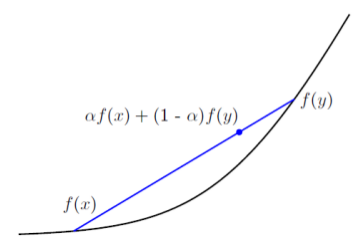
\includegraphics[width=.45\textwidth]{2018-03-04-22-09-28.png} 
	\caption{Convex Function}
	\end{figure}

\end{frame}
\begin{frame}{Convexity condition 1} 
	\begin{thm}
		Suppose $f:\real^n \rightarrow \real$ is differentiable. Then $f$ is convex if and only if for all $x,y \in \text{dom } f$. 
		$$f(y) \ge f(x) + \nabla f(x)^T (y-x) $$
	\end{thm}
	\begin{figure}
		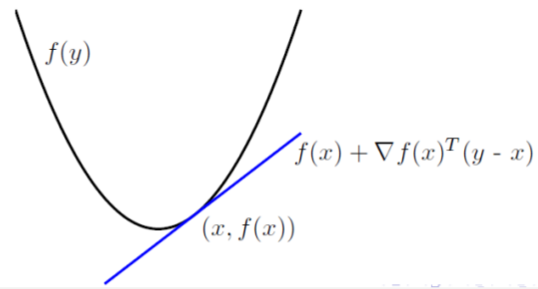
\includegraphics[width=.45\textwidth]{2018-03-04-22-24-12.png} 
		\end{figure}
\end{frame}
\begin{frame}{Subgradient}
	\begin{define}
		The \textit{subgradient} set, or subdifferential set, $\partial f(x)$ of f at x is $$\partial f(x) = \{ g: f(y) \ge f(x) +g^T(y-x) \forall y\}$$. 
	\end{define}
	
	\begin{minipage}{\textwidth}
		\begin{minipage}{.47\textwidth}
			\begin{thm}
				$f:\real^n\rightarrow \real$ is convex iff it has ono-empty subdifferential set everywhere. 
			\end{thm}
		\end{minipage}
		\hfill
		\begin{minipage}{.47\textwidth}
			\begin{figure}
				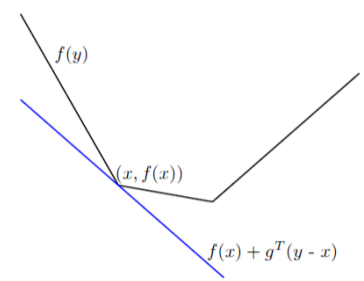
\includegraphics[width=\textwidth]{2018-03-04-22-37-40.png} 
			\end{figure}
		\end{minipage}
	\end{minipage}
\end{frame} 
\begin{frame}{Convexity condition 2} 
	\begin{thm}
		
	\end{thm}
\end{frame}
\subsection{Convex optimization} 

\section{Unconstrained optimization} 
\subsection{Gradient descent} 
\subsection{Newton's method} 
\subsection{Batch vs online learning} 
\begin{frame}{Batch gradient descent} 
	Minimize empirical loss, assuming it's convex and unconstrained 
	\begin{itemize}
		\item Gradient descent on the empirical loss: 
		\item At each step, 
		$$w^{k+1} \leftarrow w^{k} - \eta_t 
		\left( \frac{1}{n} \sum_{i=1}^{n}
		 \frac{\partial L(w,x_i,y_i)}{\partial w} \right) $$
		\item Note: at each step, gradient is the averageof the gradient for all samples $(i=1,...,n$. 
		\item Very slow when n  is very large. 
	\end{itemize}
	
\end{frame}

\subsection{Stochastic Gradient Descent} 
\begin{frame}{Stochastic Gradient Descent} 
	\begin{itemize}
		\item Alternative: compute gradient from just one (or a few samples) 
		\item Known as SGD: At each step, 
		\[ w^{k+1} \leftarrow w^{k} - \eta_t \frac{L(w,x_i,y_i)}{w}  \] 
		(choose one sample i and compute gradient for that sample only) 
		\item the gradient of one random sample is not the gradient of the objective function. 
		\item Q1:Would this work at all? 
		\item Q2: How good is it? 
		\item<2-> A1: SGD converges to not only thy empirical loss minimum, but also to the expected loss minimum! 
		\item<2-> A2: Convergence (to expected loss) is slow: $f(w_t) -E[f(w*)] \le O(1/t) $ or $O(1/\sqrt{t}) $
	\end{itemize}
\end{frame}

\begin{frame}{Practically speaking ... }
	\begin{itemize}
		\item If the training set is small, we should use batch learning using quasi-Newton or conjugate gradient descent. 
		\item If the training set is large, we should use SGD. 
		\item If the size of training set is somewhere in between, we use mini-batch SGD. 
		\item Convergence is very sensitive to learning rate, which needs to be determined by trial-and-error (model selection or cross-validation) 
	\end{itemize}
\end{frame}
\section{Constrained optimization} 
\subsection{Lagrange duality} 

\begin{frame}{Lagrangian function} 
	Start with optimization Problem: 
	\begin{equation}
		\begin{aligned}
			\min_x \quad & f_0(x)  \\ 
			\textrm{s.t.} \quad & f_i(x) \le 0, i = \{1,...,k\} \\  
					 \quad & h_j(x) = 0, j = \{1,...,l\} \\ 
		\end{aligned}
	\end{equation}
	From \emph{Lagrangian} using Lagrange multipliers $\lambda_i \ge 0, \nu_i \in \real$ 
	\begin{equation}
		\cL(x,\lambda,\nu) = f_0(x)+\sum_{i=1}^{k} \lambda_i f_i(x) + \sum_{j=1}^{l} \nu_j h_j (x) 
	\end{equation}
\end{frame}

\begin{frame}
	{Lagrangian function}
	Original/primal problem: 
	\begin{equation*}
		\begin{aligned}
			\min_x \quad & f_0(x)  \\ 
			\textrm{s.t.} \quad & f_i(x) \le 0, i = \{1,...,k\} \\  
					 \quad & h_j(x) = 0, j = \{1,...,l\} \\ 
		\end{aligned}
	\end{equation*}
	is equivalent to min-max optimization: 
	\[\min_x [\sup_{\lambda \ge 0, \nu} \cL(x,\lambda, \nu)] \]
\end{frame}

\subsection{SVM in primal and dual forms}
\subsection{Constrained methods} 

%\begin{frame}[t, allowframebreaks]
%\frametitle{References}
%
%
%\printbibliography
%\end{frame}

\begin{frame}
\chuhao Thank you! %\fontspec{LHANDW.TTF}
\end{frame}
		
	
\end{document} 